%%=============================================================================
%% Methodologie
%%=============================================================================

\chapter{\IfLanguageName{dutch}{Methodologie}{Methodology}}
\label{ch:methodologie}

Aan de hand van verschillende \acrshort{rpa} providers zal een concreet proces geautomatiseerd worden op MetaMaze. MetaMaze is een \acrfull{adp} tool ontwikkeld door Faktion. De code voor de verschillende workflows en packages geschreven voor dit onderzoek zijn te vinden op GitHub\footnote{https://github.com/MoutPessemier/BachelorProef}. Aan de hand van de uitwerking van dit proces worden de verschillende platformen gequoteerd. Deze score is een indicator hoe professioneel en gebruiksvriendelijk elk van de onderzochte platformen zijn.

Het onderzoek werd gestart vanuit het perspectief van een beginnende \acrshort{rpa} ontwikkelaar. De ervaring rond het werken met de verschillende \acrshort{rpa} providers kan sterk verschillen met een ervaren developer.


\section{Voorbereiding}
Eerst en vooral is het MetaMaze platform grondig geëxploreerd geweest. Zo werd een nieuw project aangemaakt, werden er documenten geüpload en gelabeld om een model te kunnen trainen. Nadien werd dit model dan gebruikt om voorspellingen te doen op nieuwe, soortgelijke documenten. Hierbij werd soms doelbewust een verkeerd document geüpload om ook de manuele interventie te testen en te kijken hoe dit eventueel in een proces kan gegoten worden. Op basis hiervan werd een algemeen voorbeeld proces opgezet.

Als tweede stap is de afweging gemaakt welke providers vergeleken gingen worden. Hierbij werd rekening gehouden dat er twee grote marktspelers, twee kleine en een provider die de implementatie van \acrshort{rpa} op een totaal andere manier aanpakt, gekozen waren. De volgende providers werden uiteindelijk gekozen: UiPath, Automation Anywhere, WorkFusion, IntelliBot en Microsoft Flow. Hierbij zijn Uipath en Automation Anywhere de grote providers, WorkFusion en IntelliBot de kleine en Microsoft Flow als ander concept.

 Nadien werd de documentatie en cursussen van deze platformen grondig bekeken om uiteindelijk een demo proces te bekomen. De uitwerking hiervan is te zien in figuur ~\ref{fig:exampleProcess}.

\begin{figure}[h]
	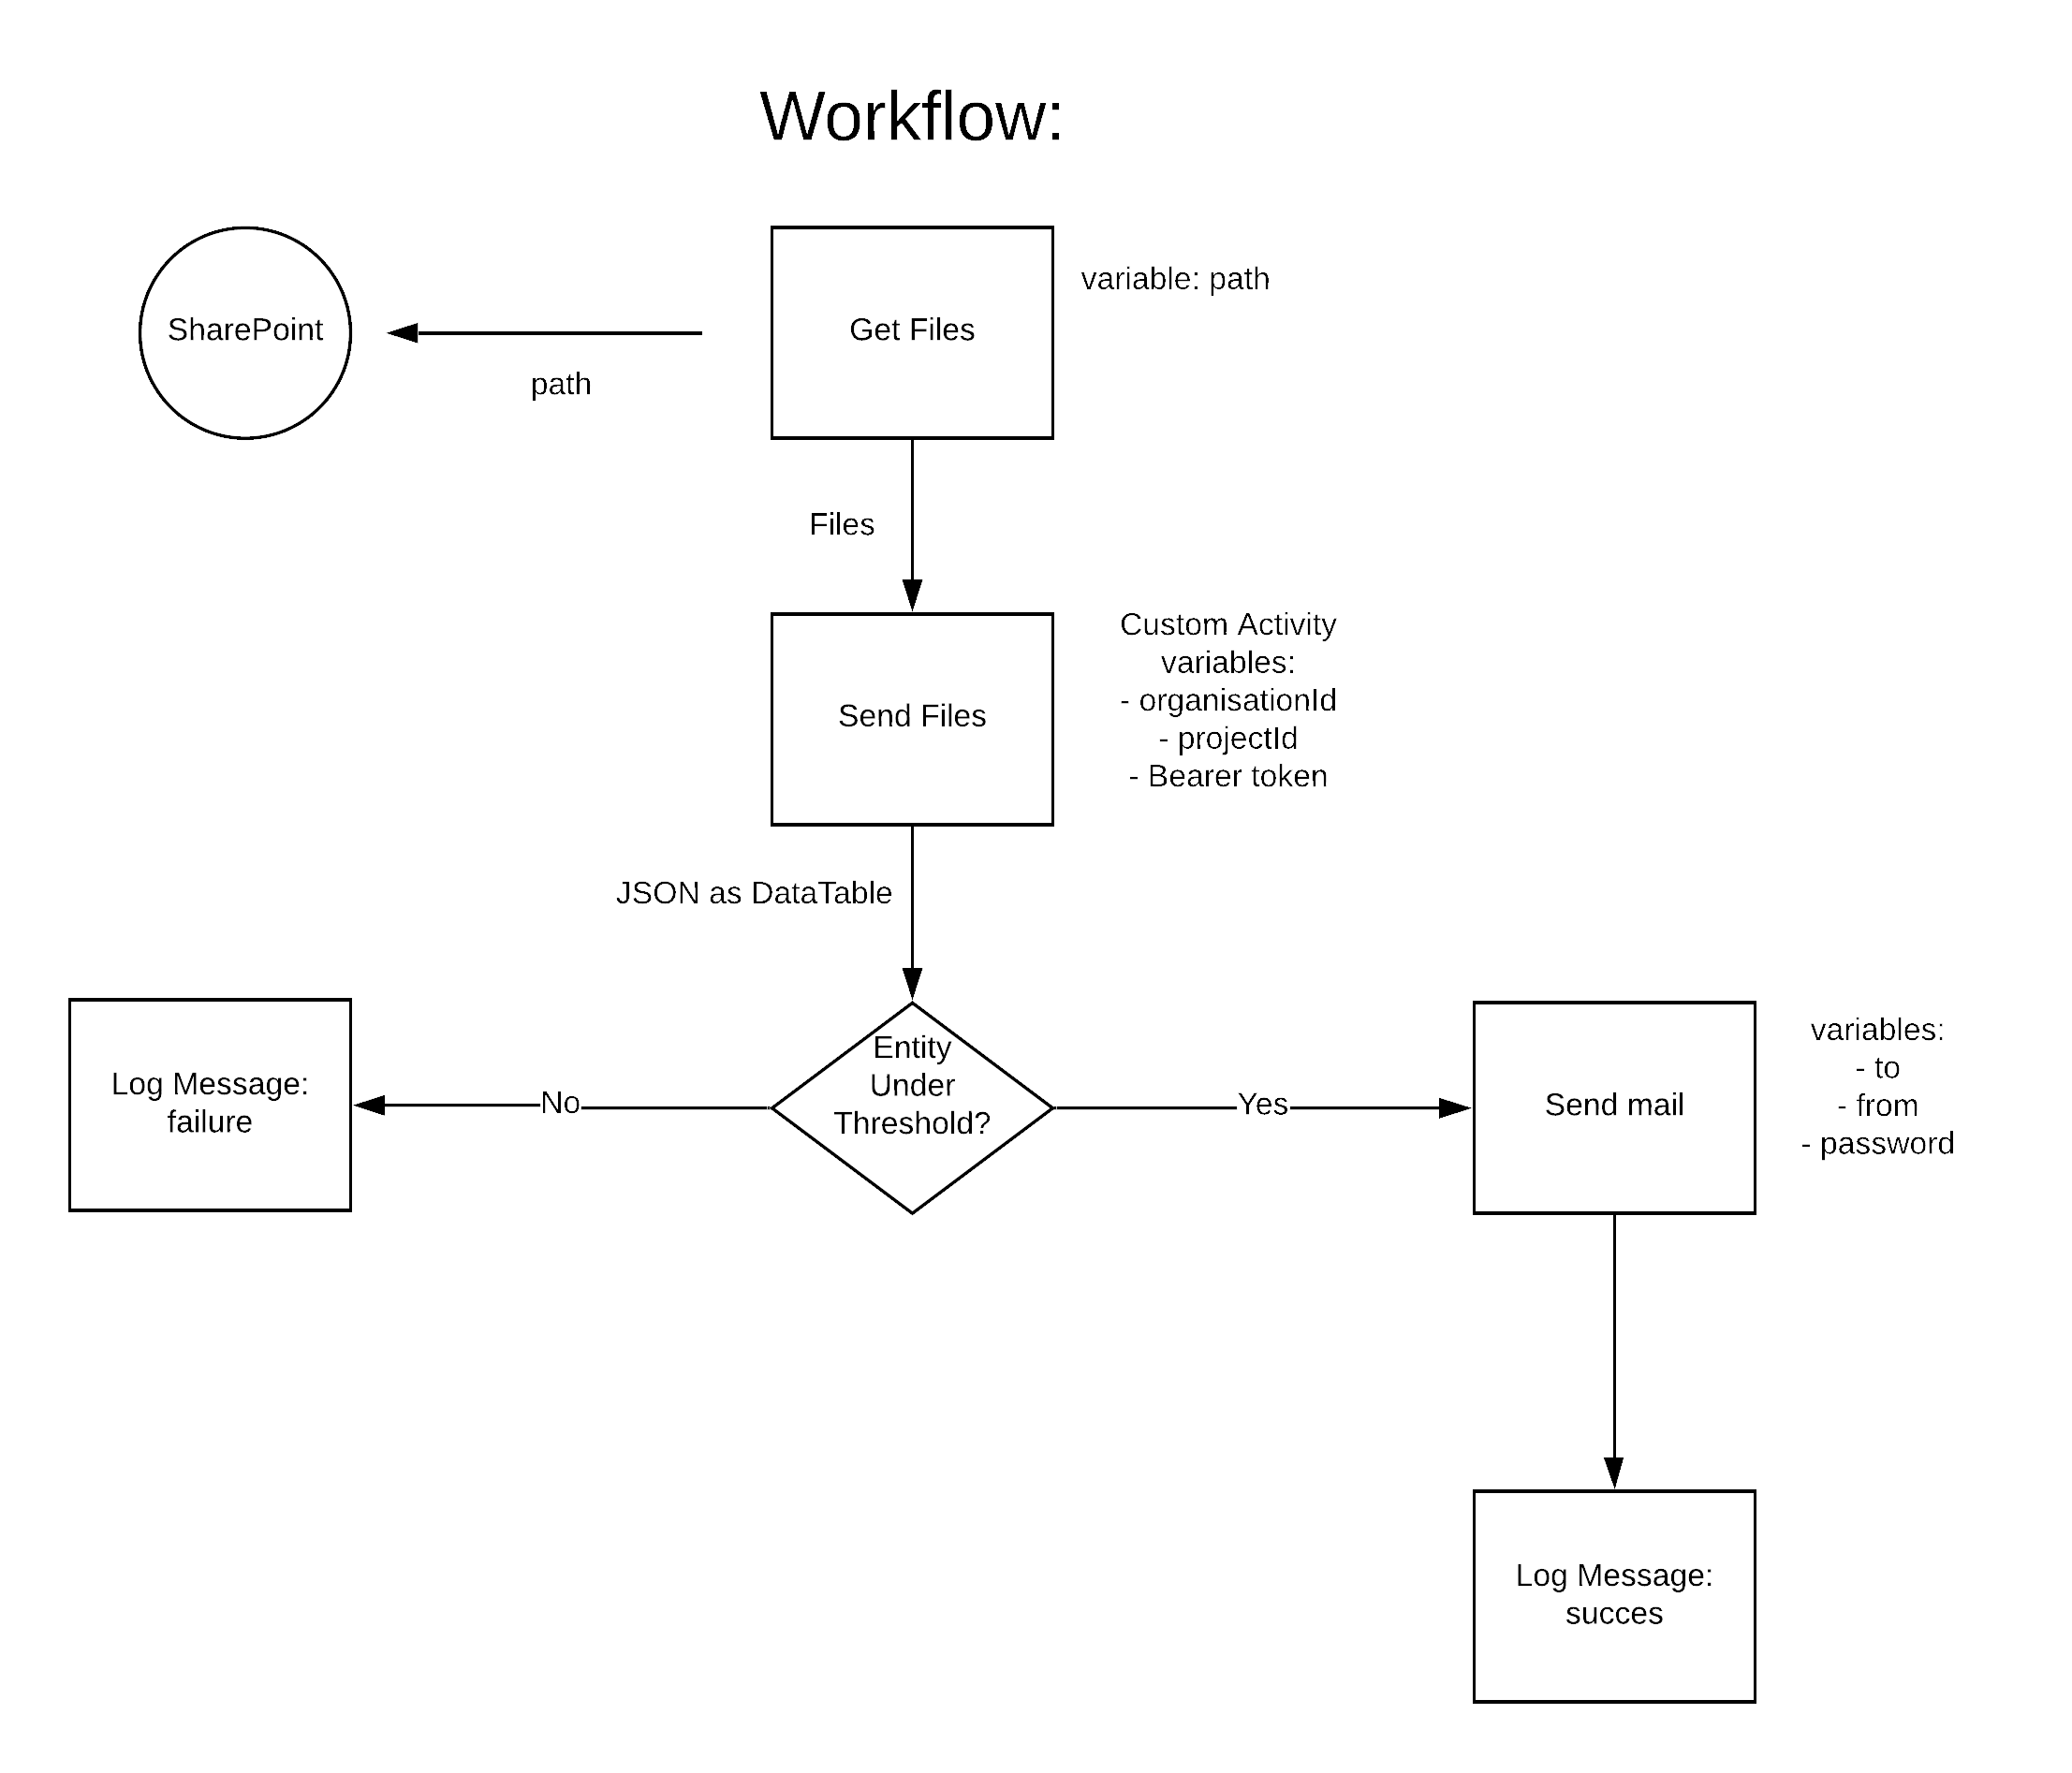
\includegraphics[width=\linewidth]{ExampleProcess.png}
	\caption[Te automatiseren demoproces]{Voorbeeldproces dat gebruik maakt van de custom Send Files \gls{activiteit}.}
	\label{fig:exampleProcess}
\end{figure}

Het algemeen proces dat zal geautomatiseerd worden op de verschillende \acrshort{rpa} solutions gaat als volgt te werk: Eerst wordt vanuit een bepaald punt (folder op de computer, OneDrive, DropBox, SharePoint) een aantal files opgehaald. Deze files worden doorgegeven aan een zelfgeschreven \gls{activiteit}. In deze \gls{activiteit} zullen deze files verstuurd worden naar de MetaMaze \acrshort{api}. De bestanden worden door de backend verwerkt. Nadien wordt er gewacht tot een antwoord terug komt van de server met de resultaten van de upload. Deze resultaten worden terug gegeven naar de volgende stap in de \gls{workflow}. Door verder te werken met de resulterende \acrshort{json} kan gekeken worden of de zekerheid waarmee een bepaalde entity dat uit een document is gehaald, onder de minimum zekerheid (threshold) zit of niet. Als er geen waarden onder de threshold zitten wordt het proces afgesloten met een gepaste melding. Als er één of meerdere confidence scores onder de threshold zitten zal eerst een mail verstuurd worden naar de klant om deze te informeren welke entities de minimum score niet gehaald hebben, voor dat het proces eindigt met een gepaste melding.

Dit is echter slechts een voorbeeldproces dat gebruikt wordt om de capaciteiten voor algemene taken zoals het versturen van een mail en werken met het bestandssysteem van de host te gaan onderzoeken.

\subsection{Criteria}
De criteria die onderzocht zijn kunnen opgedeeld worden in drie categorieën: technische criteria, bedrijfscriteria en financiële criteria.\\
Onder de technische criteria valt de mogelijkheid om zelfgeschreven \gls{activiteit}en gemakkelijk toe te voegen of te hergebruiken. Ook wordt er gekeken naar hoe het zit met de tools om de \gls{workflow}s te maken en de bots te managen. Als laatste punt wordt gekeken naar de \acrshort{ipa} capaciteiten.\\
Bij de bedrijfscriteria wordt rekening gehouden met het feit of er een grote onderneming achter het platform staat, hoe actief de community is en hoe professioneel de klantservice is.\\
Tot slot valt onder de financiële categorie de prijs van een enterprise versie maar daarnaast de mogelijkheid om een community editie te gebruiken en hoe uitgebreid deze versie is.

De nadruk wordt hier gelegd op een integratie met een eigen \acrshort{api}, op een eigen webplatform.

De verschillende criteria hebben elk een gewicht toegekend gekregen. Hierop worden ze gescoord en op het einde worden alle punten opgeteld.

\subsubsection{Puntenverdeling}
Technische Criteria
\begin{itemize}
	\item Custom activities/implementations --> is de mogelijkheid er om een eigen code toe te voegen. Als die er is, hoe uitgebreid is dit, enkel als script of ook volwaardige \gls{activiteit}en: /5
	\item Herbruikbaarheid --> kunnen bepaalde (zelfgemaakte) \gls{workflow}s/activities hergebruikt worden door jezelf en/of anderen: /3
	\item Tools --> hoe uitgebreid zijn de tools om een \gls{workflow} op te zetten: /5
	\item Bot management --> hoe en waar worden de bots gemanaged? Kan dit op een efficiënte manier: /3
	\item IPA capaciteiten --> kan \acrshort{ai} en \acrshort{ml} makkelijk geïntegreerd worden in de \gls{workflow} om IPA te bereiken. Wat wordt aangeboden door de provider zelf: /3
\end{itemize}

Bedrijfscriteria
\begin{itemize}
	\item Community --> hoe actief zijn ze op het forum, hoe groot is de community: /5
	\item Weblessen --> worden weblessen aangeboden door de provider en wat is de kwaliteit van deze lessen: /3
	\item Support --> hoe is het contact met de organisatie: /3
\end{itemize}

Financiële criteria
\begin{itemize}
	\item Prijs --> Wat is de prijs is het platform
	\item Community edition --> hoe uitgebreid en representatief is deze versie ten opzichte van de enterprise edition: /5
\end{itemize}

Dit komt uit op een totale score van 34.

\section{Implementatie}
Voor de implementatie op elk platform werd eenzelfde werkwijze gehanteerd. Eerst werd de \gls{workflow} opgebouwd rond de zelfgeschreven \gls{activiteit} om deze nadien te implementeren in de achterliggende programmeertaal van het platform. Eens deze uitgeschreven was, werd uitgezocht hoe deze \gls{activiteit}en gebruikt konden worden binnen de verschillende \gls{workflow}s.

Voor de uitwerking van de zelfgeschreven \gls{activiteit} werd eerst via pseudocode een basis uitwerking beschreven die nadien tot realisatie werd gebracht in de respectievelijke talen.

\subsection{Pseudocode}
\begin{lstlisting}
Invoer: een organisatie ID: organisationId, 
	een project ID: projectId,
	een vector van paden naar verschillende 
	bestanden om te versturen: files en een 
	bearer token om te authoriseren: bearer.
	
Uitvoer: de resulterende JSON.

1: function SendFiles(organisationId,projectId,files,bearer):
2:  client <-- HttpClient()
3:  client.authorisation <-- "Bearer " + bearer
4:  url <-- "https://x.y.z/organisationId/projectId"
5:  multiformData <-- MultiformData()
6:  foreach filePath in files do:
7:   filestream <-- fromFile(filePath)
8:   multiformData.add(filestream)
9:  end foreach
10:  try:
11:   result <-- client.post(url, multiformData)
12:  catch (exception):
13:   log(exception)
14:  end try-catch
15:  while (!response) do:
16:   try:
17:    response <-- client.get(url + result.id)
18:   catch(exception):
19:    log(exception)
20:   end try-catch
21:   end while
22:   return response
23: end function
\end{lstlisting}

Eens de pseudocode uitgedacht was, moest er slechts gezocht worden naar de juiste klassen om het proces te implementeren. Aangezien de meeste \acrshort{rpa} providers C\# gebruiken als achterliggende taal, kon over het algemeen veel code hergebruikt worden doorheen de verschillende implementaties. De overgeërfde basisklassen kan dan wel verschillen maar de algemene logica voor het versturen van een POST request en het ophalen van het resultaat met een GET request blijft dezelfde.

Tijdens het implementeren werd rekening gehouden met de verschillende criteria die vooraf vastgelegd waren.

\section{Beoordeling}
Voor de beoordeling van de prijs wordt aangeraden om te kijken naar het prijzenonderzoek, te vinden in de bijlage van deze paper.

\subsection{UiPath}
Bij UiPath is het mogelijk om in de community edition custom activities toe te voegen. Hiervoor moet een C\# Class Library gemaakt worden. Van dit project moet nadien een NuGet Package gemaakt worden en lokaal toegevoegd worden aan UiPath om toegang te krijgen tot deze \gls{activiteit}. Het nadeel hierbij is dat elke wijziging in code een nieuwe versie van de package voorstelt die opnieuw moet worden gepubliceerd. Daarnaast kan ook een VB script uitgevoerd worden. (4.5/5)

Voor de herbruikbaarheid van custom activities en \gls{workflow}s kan gebruikt gemaakt worden van de Orchestrator\footnote{https://platform.uipath.com/} in combinatie met de market place. Packages kunnen gepubliceerd worden naar de orchestrator en deze kunnen op die manier ter beschikking gesteld worden op de market zodat anderen deze package kunnen hergebruiken. Er is ook de mogelijkheid om \gls{workflow} bestanden aan te roepen binnen andere \gls{workflow}s. (3/3) 

De beschikbare tool voor het implementeren van een \gls{workflow} is UiPath Studio, een \acrfull{ide} die zich focust op het ontwerpen en uitwerken van een \gls{workflow}. Hierbinnen kan niet geprogrammeerd worden, daarvoor moet beroep gedaan worden op een C\# \acrshort{ide} zoals Visual Studio. De tool zelf voelt heel intuïtief aan en zit logisch ineen. Het is makkelijk om een \gls{workflow} op te bouwen en er zijn ook features aanwezig om de \gls{workflow} te debuggen. (5/5)

Het managen van de UiPath bots gebeurt aan de hand van het online platform, de UiPath Orchestrator. Hierop worden machines vastgelegd waarop een bot attended of unattended kan gaan werken, worden bots gedeployed, taken ingepland, queues opgezet en assets bewaard en analytics weergegeven. Kortom, alles wat nodig is om de verzameling bots te gaan managen op een professionele manier. Het platform zit logisch ineen en werkt uitstekend. (3/3)

In Studio zijn \acrshort{ocr} en Computer Vision mogelijk om te gebruiken binnen een standaard \gls{workflow} maar de echte \acrshort{ai} \gls{workflow}s moeten opgebouwd worden aan de hand van \acrshort{ai} Fabric, de tool speciaal gemaakt voor dit soort zaken. Deze zit vergrendeld achter een enterprise versie. (2/3)

De community achter UiPath is groot en actief. Het forum wordt gebruik door zowel UiPath zelf om belangrijke mededelingen te maken, als door de klanten die er terecht kunnen met vragen over allerhande topics. (5/5)

De lessen die aangeboden worden door UiPath zitten zeer goed ineen. Alles wordt rustig opgebouwd, de video's zijn duidelijk en makkelijk te volgen en er zijn voldoende oefeningen om de net geleerde skills eens te testen. (3/3).

Support zit ook goed. Ze zijn makkelijk te bereiken via ofwel het forum ofwel via mail waarop er binnen de 1-2 dagen wordt geantwoord. (2/3)

De community edition van UiPath als platform is zeer uitgebreid. In Studio kan je alles wat ook mogelijk is in de enterprise versie. Het grote verschil ligt hem in de Orchestrator. Hirbij wordt dit een on-premise (geïnstalleerd op de machine van de host) of cloud-hosted Orchestrator waarbij er een oneindig aantal robots kan gemaakt worden. Ook kunnen er meerdere soorten bots gemaakt worden. Ook wordt toegang verleend tot premium support en is er de mogelijkheid om up/down te scalen met wat nodig is binnen het bedrijf. (3/3)

Dit brengt de totale score van UiPath tot 30.5/34.

\subsection{Automation Anywhere}
Automation Anywhere staat niet toe om een custom activity te gebruiken in de community edition. Alles moet geautomatiseerd worden met de standaard \gls{activiteit}en. Het aanbod van deze reeds voorziene \gls{activiteit}en is wel uitgebreider dan bij UiPath. Voor het implementeren van een custom \gls{activiteit} kan gebruik gemaakt worden van een C\# Class Library. (3/5)

De herbruikbaarheid bij Automation Anywhere is terug te vinden in hun BotStore\footnote{https://botstore.automationanywhere.com/}. Hier kunnen bots geüpload en gedownload worden om nadien te configureren en te gebruiken. De BotStore is een equivalent van de UiPath market place. (2/3)

De tools die gebruikt worden om een \gls{workflow} te implementeren zijn allemaal cloud-based. Op de site wordt de flow opgebouwd en nadien wordt verbinding gemaakt met het lokaal apparaat waarop de \gls{workflow} getest kan worden. De tool is over het algemeen begrijpbaar maar voor eenzelfde stap in UiPath, zijn geregeld meerdere stappen nodig in Automation Anywhere. Er is ook een mogelijkheid om de \gls{workflow} te debuggen. (4/5)

Voor de bots te managen moet bij Automation Anywhere niet ver gegaan worden. Dit zit namelijk in het zelfde webplatform als het maken van de robots. Hier kunnen robots gestart worden om taken uit te voeren op bepaalde machines. Er zijn geen verschillende typen van bots. Ook de analytics zijn zichtbaar op dit platform. (1.5/3)

Voor het maken van \acrshort{ai} en \acrshort{ml} bots kan beroep gedaan worden op de IQBot van Automation Anywhere. Hier wordt de focus gelegd op \acrfull{adp} wat exact hetzelfde is als MetaMaze. Dit getrainde model kan dan gebruikt worden in een gewone flow. Daarnaast zijn er ook nog enkele standaard \gls{activiteit}en die werken met NLP en OCR. (2.5/3)

De community achter Automation Anywhere is groot en actief, al worden er geen updates gepost door Automation Anywhere zelf. Ook hier wordt gebruik gemaakt van duidelijke subcategorieën om de posts in op te delen. (4.5/5) 

Er is een zeer ruim aanbod aan lessen voor verschillende onderdelen van het \acrshort{rpa} development proces. Dit gaat van de voorbereiding tot het verstaan van de bedrijfsbehoeftes en het implementeren van een proces. De video's zijn duidelijk opgebouwd in een cursus structuur en zijn makkelijk te volgen. (3/3)

Support is lastig om in te schatten. In het begin was contact via mail of telefoon snel gelegd en er werd een inspanning geleverd om zo goed en snel mogelijk hulp te bieden op de verschillende vragen of problemen. Naargelang de tijd vorderde, verwaterde ook het contact. Dit kan natuurlijk te maken hebben met de COVID-19 crisis. (2/3)

De community editie van Automation Anywhere is uitgebreid genoeg tot het punt waar de beslissing om voor dit platform te kiezen kan gemaakt worden. Daartegenover wordt ook veel weggestoken achter de premium versie. Zo is er geen toegang tot de BotStore en zit veel van het platform en de capaciteiten om bots te gaan inplannen of taken toe te voegen, vast achter een enterprise license. Ook de IQBot zit verstopt achter een licentie. (3.5/5)

Dit levert Automation Anywhere een score op van 26/34.

\subsection{WorkFusion}

Er is geen mogelijkheid om een custom activity toe te voegen in beide versies. Wel kan een custom script geschreven worden dat code kan uitvoeren. Dit script is geschreven in Groovy en kan alleen gebruik maken van de basic Groovy onderdelen. Geen andere jar bestanden kunnen toegevoegd worden wat resulteert in zeer beperkte mogelijkheden om een eigen iets te gebruiken. (1.5/5)

Herbruikbaarheid bij WorkFusion kan gevonden worden in de recordings. Deze kunnen hergebruikt worden waarbij alleen de parameters kunnen aangepast worden. Ook kunnen functies en zelfgeschreven scripts hergebruikt worden doorheen verschillende recordings. (1.5/3)

De WorkFusion tools om een recording te maken bestaat uit een dedicated \acrlong{ide} waar zowel in kan geprogrammeerd worden als een recording opgebouwd worden. Het grootste probleem bij het programmeer gedeelte is dat er geen syntax highlighting of autocomplete is. Er moet dus feitelijk blind geprogrammeerd worden. Daarom dat meestal andere \acrshort{ide}'s gebruikt worden zoals IntelliJ. Langs de recorder kant ziet de \acrshort{ide} er zeer droog uit. De \acrfull{ui} is niet aantrekkelijk en er zijn ook maar een beperkt aantal standaard \gls{activiteit}en voorzien. (1/5)

Bot management gebeurt bij WorkFusion aan de hand van een online platform genaamd Contorl Tower. Hier worden recordings naartoe gepubliceerd. Met deze recordings wordt dan eerst een proces opgemaakt in \acrshort{bpm} stijl. Dit proces wordt dan toegekend aan een bot en nadien kan deze taak handmatig uitgevoerd worden of ingepland worden om op regelmatige tijdstippen uitgevoerd te worden. Daarnaast is er ook een credential manager en data store. (2/3)

De \acrshort{ipa} capaciteiten binnen de recording zijn zeer beperkt. Er wordt niets aangeboden rond \acrshort{ai} of \acrshort{ml}, noch rond \acrshort{nlp}. Wel kan gebruik gemaakt worden van \acrshort{ocr}. Andere \acrshort{ai} en \acrshort{ml} solutions zitten vast achter een premium account. (1/3)

De community is klein en inactief. Er gebeurd niet veel op het forum en de weinige vragen die gesteld worden, worden meestal niet opgelost. (1/5)

Er worden online lessen aangeboden maar deze zijn beperkt en niet altijd even diepgaand. Het is een start maar er mag zeker nog uitgebreid worden. (1/3)

De support is zwak. Naast het forum dat geen ondersteuning aanbiedt wordt ook zeer traag tot niet op mails gereageerd. (0.5/3)

De community edition van WorkFusion bevat enkel de \acrshort{ide}, geen toegang tot de Contorl Tower. Daarnaast geeft een premium versie ook een credential manager, task scheduler, meerdere parallel lopende bots, \acrshort{ml} capaciteit en geavanceerde analytics. (2.5/5)

Alles opgeteld komt dit uit op 12/34 voor WorkFusion.

\subsection{Intellibot}

Custom activities zijn zeer gemakelijk te schrijven voor IntelliBot en dit alles dan ook nog eens binnen de community editie. Er moet niet gebuild en gepubliceerd worden tot een package, de .dll file kan rechtstreeks gebruikt worden. Daarnaast is er ook nog eens de mogelijkheid om een script toe te voegen als een volledige class library niet nodig is. (5/5)

Er is de mogelijkheid om een \gls{activiteit} aan te roepen vanuit een \gls{workflow}. Dit staat toe om \gls{workflow}s te gaan hergebruiken. Er is geen soort markt waar klanten \gls{workflow}s op kunnen zetten voor anderen maar het is wel mogelijk om \gls{workflow}s op te slaan en te gebruiken. (1/3)

De tools gebruikt om een \gls{workflow} te bouwen in IntelliBot is hun eigen \acrshort{ide}, IntelliBot Studio. Hierin kan niet geprogrammeerd worden. Het opbouwen van de \gls{workflow} is totaal anders als de rest. Bij de andere providers was het altijd in sequentie op te bouwen en was het duidelijk welke \gls{activiteit} volgt uit welke. Bij IntelliBot is dit een pak minder overzichtelijk. Hier wordt gebruik gemaakt van lijnen om \gls{activiteit}en met elkaar te verbinden en zo de \gls{workflow} op te bouwen. Van zodra een \gls{activiteit} met veel input en output gebruikt wordt, dan wordt het snel een warboel van lijnen die door elkaar getrokken worden. Hierdoor is het makkelijk om het overzicht te verliezen. (2.5/5)

Ook IntelliBot heeft zoals UiPath een web platform, de Orchestrator\footnote{http://orchestrator.intellibot.io/}, waarop het managen van de bots plaats vindt. Beide platformen lijken op elkaar, al is die van UiPath uitgebreider en ook iets beter ineen gestoken. (2/3)

De \acrshort{ai} capaciteiten van IntelliBot zitten verweven in hun \acrfull{cmp}. Deze legt vooral de focus op het automatisch verwerken van documenten, zoals MetaMaze. Daarnaast zijn ook computer vision en enkele cognitieve \gls{activiteit}en zoals sentiment analyse beschikbaar. (2/3)

De IntelliBot community is net zoals WorkFusion beperkt in aantal maar in tegenstelling tot WorkFusion is deze wel actief. De werknemers van IntelliBot volgen het forum op en antwoorden ook op de verschillende vragen. (3/5)

De lessen aangeboden op het platform zijn inhoudelijk diepgaand genoeg maar zeer beperkt in aantal. (1.5/3)

De support is zeer goed bij IntelliBot. Ze focussen zich op de individuele klant in plaats van de massa wat soms het geval is bij de grote providers. Feedback en hulp worden voorzien op maat en binnen twee werkdagen een antwoord ontvangen is dan ook geen verrassing. (3/3)

De community editie bevat voor de IntelliBot Studio bijna elke feature. Het enigste wat vergrendeld zit achter de enterprise edition, is het maken van chatbots. Aan de andere kant is de orchestrator wel onderhevig aan grote wijzigingen. Zo kan je een bot alleen lokaal draaien in de comunity editie. Voor het inplannen van taken en het toekennen van jobs aan bots moet een premium license gekocht worden. Zelf raden ze aan om de community editie te gebruiken voor het maken en testen van robots en de enterprise editie te kopen van zodra ze naar productie moeten. (3.5/5) 

Intellibot scoort 23.5/34.

\subsection{Microsoft Flow}

Custom connectors kunnen geschreven worden als een \acrshort{api} die de Open\acrshort{api} standaarden volgt of als een Azure Function. Uit deze definitie kan dan de custom connector gemaakt worden en gebruikt worden in de verschillende \gls{workflow}s. Ook vanuit Azure Functions kunnen deze custom connectors gedefinieerd worden. In begin is dit zeker niet makkelijk maar eens de samenhang en de beide platformen duidelijk worden, kan dit gemakkelijk geïmplementeerd worden. (3.5/5)

Custom Connectors kunnen herbruikt worden binnen meerdere flows. Ook kunnen ze verspreid worden naar andere klanten door de connector te publishen. Hiervoor moet door een validatie proces gegaan worden waarbij de custom connector getest moet worden en nadien gepubliceerd wordt. (2/3)

De tool die gebruikt word om de \gls{workflow} te maken is het web platform. Hierbinnen kunnen verschillende triggers en connectoren gebruikt worden om een flow op te bouwen. De layout is zeer proper, alles is duidelijk en zit logisch ineen. (4/5)

Voor het managen van bots bij Power Automate kan op dezelfde site gebleven worden. Het manueel uitvoeren van een bot gebeurd op de site, de andere soort robots zijn trigger-based. Dit wil zeggen dat ze automatisch uitgevoerd worden als een bepaalde conditie voldaan is zoals een nieuwe file in een folder toevoegen of het sturen van een \acrshort{http} request. (1.5/3)

Wanneer gekeken wordt naar de \acrshort{ai} capaciteiten, dan zijn er connectors die \acrshort{ai} en \acrshort{ml} platformen gaan aanspreken. Daarnaast hebben ze ook een \acrshort{ai} Builder die kan gebruikt worden om modellen te trainen en functies zoals sentiment analyse, taaldetectie, tekstherkenning, object herkenning en voorspellingen te maken. Deze zit ook vast achter een premium account. (2.5/3)

De community achter Power Automate en Flow is groot en actief. Het forum wordt niet gebruikt door Microsoft zelf om belangrijke aankondigingen te maken. (4/5)

Microsoft biedt zelf geen lessen aan, er zijn wel vele lessen online terug te vinden. (0/3)

Support is zeer zwak, zelfs de premium versie ervan. Zeer trage hulpverlening en reacties die geregeld niet helpen. (0.5/3)

De community editie is extreem beperkt. Bijna elke connector vereist een premium account en bij de gratis connectoren zitten er vele tussen die gebruik maken van een gateway of andere feature waarvoor je opnieuw een premium account nodig hebt. Zonder premium is het praktisch onmogelijk om een proces succesvol te automatiseren (0.5/5)

Microsoft Flow behaalt een score van 18.5/34.


\subsubsection{Algemene opmerking}
Waar sommige \acrshort{rpa} providers punten verloren hebben op bepaalde aspecten omdat ze nog klein zijn in schaal of community, wilt niet zeggen dat ze daarom slecht zijn. Ze hebben grote concurrenten om tegen op te boksen en met genoeg tijd kan hun platform ook uitgroeien tot een van de grote/beste providers.

\subsection{Samenvattende Tabel}
\begin{sidewaystable}[h!]
	\centering
	\begin{tabular}{|c||c|c|c|c|c|}
		\hline
		& \textbf{UiPath} & \textbf{\makecell{Automation\\Anywhere}} & \textbf{WorkFusion} & \textbf{IntelliBot} & \textbf{\makecell{Microsoft\\Flow}} \\
		\hline
		\hline
		Custom Activities & community & enterprise & community & community & community \\
		\hline
		Herbruikbaarheid & \makecell{NuGet package \&\\Orchestrator}  & BotStore & \makecell{Recordings zijn\\herbruikbaar} & \makecell{invokeren\\van \gls{workflow}s} & \makecell{publiceer\\connectors} \\
		\hline
		Tools & \makecell{UiPath\\Studio} & \makecell{Web\\platform} & \makecell{Workfusion\\Intelligent\\Automation\\Cloud} & \makecell{IntelliBot\\Studio} & \makecell{Web\\platform} \\
		\hline
		Type \acrshort{rpa} & \makecell{\gls{low_code_rpa}\\visual based} & Script based & \gls{no_code_rpa} & \gls{no_code_rpa} & \gls{no_code_rpa} \\
		\hline
		Bot management & Orchestrator & \makecell{All-in-on\\webplatform} & Control Tower & Orchestrator & \makecell{All-in-on\\webplatform} \\
		\hline
		IPA capaciteiten & \acrshort{ai} Fabric & IQBot & \makecell{enkele\\\gls{activiteit}en} & \acrshort{cmp} & \acrshort{ai} Builder   \\
		\hline
		Community & \makecell{Groot \&\\actief} & \makecell{Groot \&\\actief} & \makecell{Klein \&\\inactief} & \makecell{Klein \&\\actief} & \makecell{Groot \&\\actief} \\
		\hline
		Weblessen & ja & ja & ja & ja & nee \\
		\hline
		Support & Goed & Goed & Zeer zwak & Zeer sterk & Zeer zwak \\
		\hline
		Community Edition & Uitgebreid & Uitgebreid & Doenbaar & Uitgebreid & Zeer beperkt \\
		\hline
		\makecell{Onderliggende\\Technologie} & C\# & C\#/Java & Groovy & C\# & C\# \\
		\hline
		\hline
		Score & 30.5/34 & 26/34 & 12/34 & 23.5/34 & 18.5/34 \\
		\hline
	\end{tabular}
	\caption{Vergelijking van de verschillende \acrshort{rpa} Providers.}
	\label{Vergelijking}
\end{sidewaystable}
